\normalfalse \difficiletrue \tdifficilefalse
\correctionfalse

%\UPSTIidClasse{11} % 11 sup, 12 spé
%\newcommand{\UPSTIidClasse}{12}

\exer{Chariot élévateur de bateaux $\star\star$ \label{C2:09:49}}

\setcounter{question}{0}\UPSTIcompetence[2]{C2-09}
\index{Compétence C2-09}
\index{TEC}
\index{Théorème de l'énergie cinétique}
\index{Chariot élévateur de bateaux}
\ifcorrection
\else
\marginnote{\textbf{Pas de corrigé pour cet exercice.}}
\fi

\ifprof
\else

L’objectif est d’obtenir un modèle dynamique du mécanisme de basculement à partir de la modélisation plane proposée sur la figure suivante.


\begin{center}
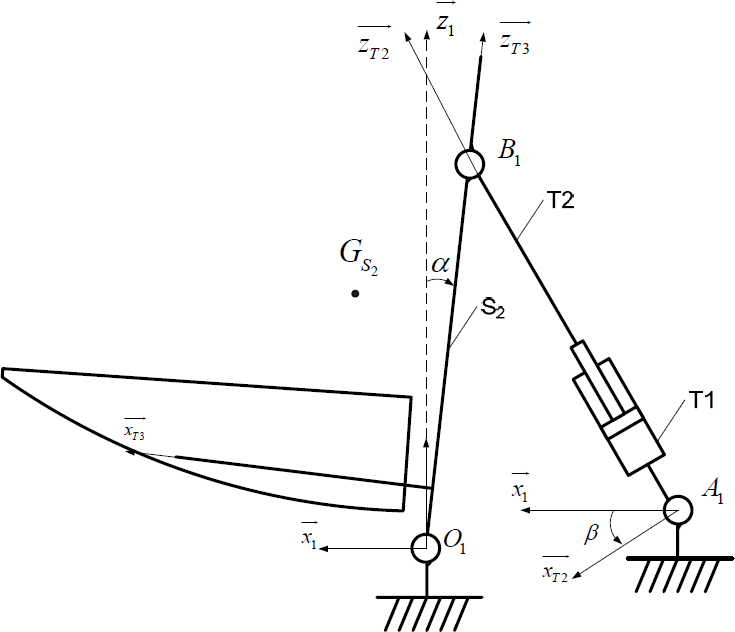
\includegraphics[width=\linewidth]{49_01}
\end{center}

Les solides pris en compte pour l’étude sont :
\begin{itemize}
\item l'ensemble $S_2$=\{ T3, T4, T5, T6, T7, T8, T9, T10, T11, B\} en liaison pivot d'axe $\axe{O_1}{y_0}$ par rapport au chariot 1 de centre de gravité $G_{S_2}$. Le moment d’inertie de l’ensemble $S_2$ par rapport à l’axe sera $\axe{G_{S_2}}{y_1}$ noté $J_{S2}$ et sa masse $m_{S2}$. La liaison pivot entre l’ensemble $S_2$ et le chariot génère un couple résistant $\vect{C_{\mu}}=-\mu\dot{\alpha}\vect{y_0}$ et $\vect{O_1O_{G_{S2}}}=x_{G_{S2}} \vect{x_{T3}}+z_{G_{S2}} \vect{z_{T3}}$; 
\item un vérin équivalent $V=\left\{ T1,T2\right\}$ dont la tige est en liaison pivot d’axe $\axe{A_1}{y_0}$ par rapport au chariot 1 et le corps en liaison pivot d’axe $\axe{B_1}{y_0}$ par rapport à l’ensemble $S_2$. La masse et l’inertie du vérin sont négligées. Le vérin développe un effort au cours du mouvement qui sera noté $\vect{F_V} = p(t) S \vect{z_{T2}}$ où $p(t)$ est la différence de pression entre les deux chambres du vérin.
\end{itemize}


On pose $\vect{A_1B_1} = \left( \lambda_0+\lambda\right)\vect{z_{T2}}$. Le paramétrage est tel que si $\alpha=0$ alors $\lambda=0$.
\fi



\question{Tracer le graphe des liaisons.}
\ifprof
\begin{center}
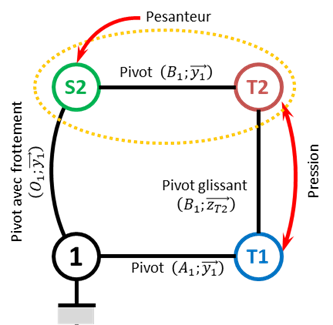
\includegraphics[width=.5\linewidth]{49_02}
\end{center}

\else
\fi

\question{En appliquant le théorème de l’énergie-puissance et en admettant que l’angle $\alpha$ est petit, montrer que $\alpha(t)$ et $p(t)$ sont liés par l’équation différentielle suivante :  $J_{\text{eq}}\ddot{\alpha}(t) + \mu \dot{\alpha}(t) =\dfrac{Sp(t)}{k}+m_{S_2}g x_{G_{S_2}}$. Exprimer $J_{\text{eq}}$.}
\ifprof

	 On isole l'ensemble $E=\{S2 ; T2,\}$. On applique le théorème de l’énergie cinétique à l’ensemble en mouvement dans le référentiel terrestre galiléen : 
	 $\mathcal{P}_{\text{int}}(E)+\pext{\overline{E}}{E}{R_g} = \dfrac{\dd \ec{E}{R_g} }{\dd t}$.

\textbf{Calcul des puissances externes}

$\pext{\text{pes}}{2}{R_g} = $

%	P(pes→S_2⁄1)={█(-m_(S_2 ) g(z_1 ) ⃗@0 ⃗ )}_(G_(S_2 ) )⊗{█((Ω(S_2⁄1) ) ⃗=α ̇(y_1 ) ⃗@(V(G_(S_2 ),S_2⁄1) ) ⃗=-x_(G_(S_2 ) ) α ̇(z_(T_3 ) ) ⃗+z_(G_(S_2 ) ) α ̇(x_(T_3 ) ) ⃗ )}_(G_S2 )=(-m_(S_2 ) g(z_1 ) ⃗ )⋅(-x_(G_(S_2 ) ) α ̇(z_(T_3 ) ) ⃗+z_(G_(S_2 ) ) α ̇(x_(T_3 ) ) ⃗ )=-m_(S_2 ) g(-x_(G_(S_2 ) ) α ̇ cos⁡α+z_(G_(S_2 ) ) α ̇ sin⁡α )
%	(V(G_(S_2 ),S_2⁄1) ) ⃗=(V(O_1,S_2⁄1) ) ⃗-(x_(G_(S_2 ) ) (x_(T_3 ) ) ⃗+z_(G_(S_2 ) ) (z_(T_3 ) ) ⃗ )∧α ̇(y_1 ) ⃗=-x_(G_(S_2 ) ) α ̇(z_(T_3 ) ) ⃗+z_(G_(S_2 ) ) α ̇(x_(T_3 ) ) ⃗
%	P(1→S_2⁄1)={█(-@L_12 (x_1 ) ⃗-μα ̇(y_1 ) ⃗+N_12 (z_1 ) ⃗ )}_(O_1 )⊗{█(α ̇(y_1 ) ⃗@0 ⃗ )}_(O_1 )=-μα ̇^2	 
%	P(T_1→T_2⁄1)_(pivot glissant)=0 (pivot glissant sans frottement)
%	P(T_1→T_2⁄1)_vérin={█(p(t)S(z_(T_2 ) ) ⃗@ -)}_(B_1 )⊗{█(0 ⃗@λ ̇(z_(T_2 ) ) ⃗ )}_(B_1 )=p(t)Sλ ̇=p(t)Sα ̇/k
%	P(E ̅→E⁄R_g )=-m_(S_2 ) g(-x_(G_(S_2 ) ) α ̇ cos⁡α+z_(G_(S_2 ) ) α ̇ sin⁡α )-μα ̇^2+p(t)Sα ̇/k

\textbf{	Calcul des puissances internes}
 $\mathcal{P}_{\text{int}}(E)=0$ car pas de frottement dans la liaison pivot.
%	Calcul de l'énergie cinétique de l'ensemble : seules la masse et l’inertie de S2 sont à prendre en contact (elles sont négligeables pour T2). E_c (S_2⁄1)=1/2 J_S2 α ̇^2+1/2 m_S2 (V_(G_S2,S_2⁄1) ) ⃗^2=1/2 (J_(S_2 )+m_(S_2 ) (x_(G_(S_2 ))^2+z_(G_(S_2 ))^2 )) (α^2 ) ̇=1/2 J_eq (α^2 ) ̇
%avec J_eq=J_(S_2 )+m_(S_2 ) (x_(G_(S_2 ))^2+z_(G_(S_2 ))^2 ). 
%On trouve donc, au final :
%J_eq α ̈+μα ̇=p(t)S/k+m_S2 g(x_(G_S2 )  cos⁡α-z_(G_S2 )  sin⁡α )  
%Si on suppose l'angle αnul (situation de la question précédente), on retrouve bien l'expression demandée.


\else
\fi






\ifprof
\else
\begin{flushright}
\footnotesize{Corrigé  voir \ref{C2:09:49}.}
\end{flushright}%
\fi